% Report
\documentclass[10pt,journal]{IEEEtran}

% Packages
\usepackage{amsfonts}
\usepackage{amsmath}
\usepackage{algorithm}
\usepackage{algorithmic}
\usepackage{amssymb}
\usepackage{graphicx}
	\graphicspath{{F:/校文件/数学/线性代数/Project/Figures/}}
\usepackage{cite}
\usepackage{subfigure}
\usepackage{float}
\usepackage{color}
\usepackage[colorlinks, linkcolor = red]{hyperref}
\usepackage{array}
		\makeatletter
		\newcommand{\thickhline}{%
			\noalign {\ifnum 0=`}\fi \hrule height 1pt
			\futurelet \reserved@a \@xhline
		}
		\newcolumntype{"}{@{\hskip\tabcolsep\vrule width 1pt\hskip\tabcolsep}}
		\makeatother

\renewcommand{\[}{\begin{equation*} \begin{aligned}} % substitute `\[`, `\]` for aligned equations
	\renewcommand{\]}{\end{aligned} \end{equation*}}

\begin{document}

% Title
\title{SI131 Final Report On \\Sparse Representation Based Face Recognition}
\author{\IEEEauthorblockN{Guanzhou Hu}\\
\IEEEauthorblockA{School of Information Science and Technology\\
  ShanghaiTech University}} 
\maketitle

% Abstract
\begin{abstract}
This report focuses on sparse representation based face recognition. Grayscale face images of different people are given for training and testing. Mathematical formulation will be proposed in the first stage, followed by \textit{Matlab} programming realization of the algorithm. Performances under different parameter tunings will then be demonstrated. Future improvements and observations are stated in the last section.
\end{abstract}

% Problem Formulation
\section{\textbf{\large Problem Formulation}}
For computers, grayscale face images are not seen as a whole ``picture'', but a $2$-dimensional array with each element ranging from $0$ to $255$. To accomplish the task of learning what are the features of a human face, it will be supplied with face images of certain individuals (several images for each person). \\

Using these training data, the program extracts the outstanding features among all images (stored in matrix $\mathbf{A}$). When given a test image $\mathbf{y}$, it solves the following linear system
\[
	\mathbf{y = Ax +e}
\]
where $\mathbf{e}$ is the error we want to minimize and $\mathbf{x}$ a vector containing coefficients of corresponding features in $\mathbf{A}$. By observing $\mathbf{x}$, the program is able to determine which individual the test image $\mathbf{y}$ belongs to.

% Algorithm
\section{\textbf{\large Algorithm}}
Images represented by data can be huge in size. Consider a typical $1920 \times 1080$ size wallpaper for your laptop desktop. It contains $1920 \times 1080 = 2.07 \times 10^6$ pixels. Given a bunch of face images, if we view every tiny pixel as a feature dimension, the analysis may require huge amount of computation and is incredibly low in efficiency. In order to reduce the redundant features and highlight the principle features, principle component analysis (PCA) is introduced to our algorithm. \\

This sparse representation based face recognition algorithm runs the following procedures.
\begin{enumerate}
	\item \textit{Data Reading}
	\item \textit{Training Data Processing}
	\item \textit{Principle Component Analysis on Training Data}
	\item \textit{Testing Data Renormalization}
	\item \textit{Recognition Accuracy Testing}
\end{enumerate}

%%
\subsection{\large Data Reading}
For each individual, $numTrainee$ (set by user) pieces of training photos and $numTestee = 15$ pieces of testing photos are randomly choosen. Every image is converted from a $2$-dimensional matrix $\mathbf{I}$ into an image vector $\mathbf{v}$, by concatenating each column vector end to end, left to right, as demonstrated below.
\[
	\mathbf{I} = \begin{bmatrix}
		p_{1,1} & \cdots & p_{1,w} \\
		\vdots & \ddots & \vdots \\
		p_{h,1} & \cdots & p_{h,w}
	\end{bmatrix} \in \mathbb{R}^{h \times w} \Rightarrow \mathbf{v} = \begin{bmatrix}
		p_1 \\
		\vdots \\
		p_{wh}
	\end{bmatrix} \in \mathbb{R}^{wh}
\]

By putting all training image vectors as column vectors, we get the training image matrix $\mathbf{T}$. Each column of it is a sample (or called obvservation), and each row is a feature variable. Denote the total number of training samples as $s$. Similar procedure for the testing image matrix $\mathbf{Y}$, and total number of testing samples is $t$.

%% 
\subsection{\large Training Data Processing}
In order to normalize the input data, we divide each column of $\mathbf{T}$ by its L2-Norm, 
\[
	\mathbf{T}(i) \ /= \ ||\mathbf{T}(i)||_2
\]
for all $i$, so that every sample is normalized as a unit vector. Same for testing data $\mathbf{Y}$. Mean value of every feature is also computed as put into mean vector $\mathbf{meanT}$.

%% 
\subsection{\large Principle Component Analysis on Training Data}
The core of this algorithm is to use PCA to lower the feature dimension, in order to increase the efficiency of computation meanwhile maintain a high rate of information. We first shift every sample in matrix $\mathbf{T}$ to zero mean, getting standardized $\mathbf{B}$. \\

In the next stage, we need to compute the covariance matrix $\mathbf{covB}$ representing the relationships between features of $\mathbf{B}$,
\[
	\mathbf{covB} = \frac{\mathbf{B B^T}}{s-1}
\]
whose eigenvectors give a new basis, where data is mainly distributed at several base vector directions. The original algorithm computes these eigenvectors by decomposing $\mathbf{B B^T}$ directly. However, noticing that $\mathbf{B} \in \mathbb{R}^{wh \times s}$, the covariance matrix will be size $wh \times wh$, which is definitely not suitable for computing eigenvectors and eigenvalues. From the insight that matrix transposing and Spectral Decomposition (SD) are tightly related \cite{cnki1}, we compute eigenvectors of the matrix $\mathbf{B^T B}$ which is size $s \times s$ -- much smaller than the covariance matrix,
\[
	\mathbf{B^T B x} = \lambda \mathbf{x}
\]
and by the mathematical relationships below,
\[
	\mathbf{B B^T B x} = \mathbf{B} \lambda \mathbf{x}
\]
we see that vector $\mathbf{B x}$ is an eigenvector of $\mathbf{covB}$. Therefore, after we require the eigenvector matrix $\mathbf{V}$ and eigenvalue array $\mathbf{d}$ for $\mathbf{B^T B}$, we extract the largest $k$ eigenvalues satisfying 95\% accuracy
\[
	\frac{\sum^k \lambda_{selected}}{\sum_{i=1}^s \lambda_i} \ge 0.95
\]
and their corresponding eigenvectors $\mathbf{V_k}$. Then we simply acquire the principle eigenvector matrix $\mathbf{COEFF}$ for $\mathbf{covB}$ by
\[
	\mathbf{COEFF = B V_k}
\]
Notice that $\mathbf{COEFF}$ is not necessarily unitized now, therefore we divide each eigenvector by its L2-Norm to obtain unit bases of the principle components
\[
	\mathbf{COEFF}(i) \ /= \ ||\mathbf{COEFF}(i)||_2
\]
for $i \in \{1, 2, \dots , k\}$. \\

$\mathbf{COEFF}$ is the bases of principle subspace that we project the data $\mathbf{B}$ on. After change of basis, the data goes into coefficients $\mathbf{pcaT}$ under the new basis
\[
	\mathbf{pcaT = COEFF^T * B}
\]

%% 
\subsection{\large Testing Data Renormalization}
As a premise of comparison, the testing images must also be projected onto the principle eigen-subspace. We have already make testing data $\mathbf{Y}$ a normalized matrix. Then we subtract the mean of training data $\mathbf{meanT}$ from $\mathbf{Y}$ and change its basis
\[
	\mathbf{pcaY = COEFF^T * (Y} - rep(\mathbf{meanT}))
\]
to acquire the comparative testing data $\mathbf{pcaY}$, whose columns represent testing face images of an individual.

%% 
\subsection{\large Recognition Accuracy Testing}
For every test image $\mathbf{y}$, i.e. a column of $\mathbf{pcaY}$, the \textit{ideal} condition is that it can be represented as a linear combination of all training images, with respective to the principle features:
\[
 	\mathbf{y} = x_1 \mathbf{v_{pca, 1}} + x_2 \mathbf{v_{pca, 2}} + \cdots + x_s \mathbf{v_{pca, s}}
\]
where $\mathbf{x} = (x_1, x_2, \dots , x_s)$ is a sparse vector, such that, if the large coefficients concentrate at a certain individual, it reveals the possible face this test image belongs to. \\

We aim to minimize the error $\mathbf{e = y - pcaT * x}$, and also need to keep $\mathbf{x}$ as sparse as possible. Therefore, the equation we have to solve is
\[
	\hat{\mathbf{x}} = arg \min_{\mathbf{x}} \frac{1}{2} ||\mathbf{y - pcaT * x}||_2^2 + \lambda ||\mathbf{x}||_1
\]
where $\lambda$ needs to be tuned to obtain the best result. Using $feature\_sign()$ linear solver, for every test image, the coefficients $\mathbf{x}$ is computed. \\

Instead of directly choosing the result to be the face with maximum coefficient, we gather all $numTrainee$ coefficients for each individual, computes their L2-Norm $x\_norm$ and pick the face with maximum $x\_norm$ as the final classification. Accuracy of recognition is defined by
\[
	\text{ACCURACY} = \frac{\text{number of correct tests}}{t}
\]

% Dataset Description
\section{\textbf{\large Dataset Description}}
The dataset \textit{CroppedYale} I use contains $38$ different individuals and $57 \sim 64$ valid face images for each individual. The rule of random selection of training and testing data is as follows:
\begin{itemize}
	\item Read in $numTrainee$ from function input and set $numTestee = 15$
	\item Inside every individual's folder, generate a random permutation of $numTrainee + numTestee$ numbers
	\item Pick the first $numTrainee$ corresponding images as training data
	\item Pick the rest images in permutation as testing data; this ENSURES disjointness between training data and testing data
\end{itemize}

Each face image is grayscale and of size $192(h) \times 168(w)$ pixels. Therefore each image is represented by a length-$192 \times 168 = 32256$ vector. \\

``Mean Face'' and the largest four ``Eigen Faces'' (four most significant components) of individual \textit{yaleB01} is illustrated below for an example.
\begin{figure}[H]
	\centering
	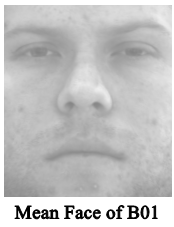
\includegraphics[width=0.3\columnwidth]{meanface.png}
\end{figure}
\begin{figure}[H]
	\centering
	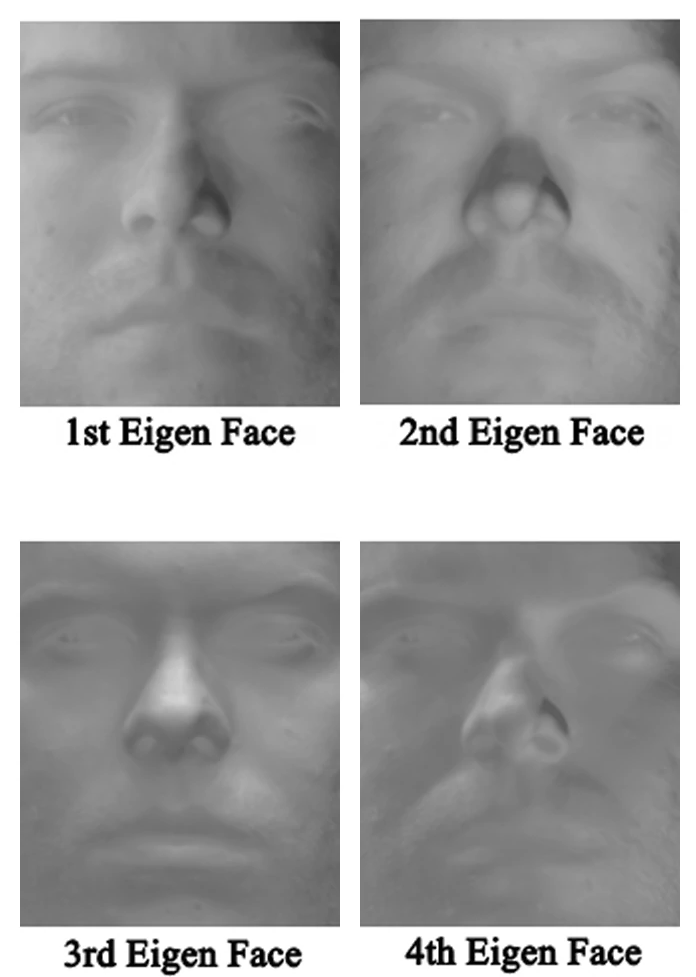
\includegraphics[width=0.6\columnwidth]{eigfaces.png}
	\caption{Dataset Illustration}
\end{figure}

% Code
\section{\textbf{\large How to Run My Code}}
All components of this algorithm is listed as follows:
\begin{itemize}
	\item SRBFR($numTrainee$, \textit{path}), the main function
	\item PCA($X$), PCA accomplishment
	\item feature\_sign($\mathbf{A, y}, \lambda, init\_\mathbf{x}$), the linear solver
	\item \textit{Cropped Yale} Dataset
\end{itemize}

Invoke SRBFR() with parameters $numTrainee$, the number of training images for each individual, and \textit{path}, the file path downto dataset folder $CroppedYale$. The return value will be accuracy of recognition.

% Performance
\section{\textbf{\large Performance}}
The actual performance of this algorithm include both \textit{Accuracy} and \textit{Efficiency}. The recognition accuracy is effected by the parameter $\lambda$ and the size of training data $numTrainee$. Also, run time is compared between official $pca()$ accomplishment and my fast $PCA()$ accomplishment. Testing environment is as Table \ref{tab:env}.
\vspace{8pt}
\begin{table}[H]
	\centering
	\begin{tabular}{cccc}
		\thickhline
		\textbf{System} & \textbf{CPU} & \textbf{Memory} & \textbf{MATLAB} \\ \hline
		Windows 10 x64 & Intel Core i7-6700HQ & 16G & R2015b \\ \thickhline
	\end{tabular}
	\vspace{6pt}
	\caption{Testing Environment} \label{tab:env}
\end{table}

%% 
\subsection{\large $\lambda$ Tuning}
Fix the number of training data $numTrainee = 40$, $\lambda$ is tuned in the range of $0.001 \sim 0.03$, and the \textit{Accuracy} result of every $\lambda$ is obtained by taking mean of $5$ tests. The result is shown in Table \ref{tab:perf1} and Figure \ref{fig:perf1}.
\vspace{8pt}
\begin{table}[H]
	\centering
	\begin{tabular}{c||cccc}
		\thickhline
		$\lambda$ & 0.001 & 0.003 & 0.005 & 0.008 \\ 
		\textit{Accuracy} & 0.9467 & 0.9537 & 0.9601 & 0.9614  \\ \hline
		$\lambda$ & 0.01 & 0.012 & 0.015 & 0.03 \\
		\textit{Accuracy} & 0.9540 & 0.9498 & 0.9477 & 0.9361 \\ \thickhline
	\end{tabular}
	\vspace{6pt}
	\caption{Result of $\lambda$ Tuning} \label{tab:perf1}
\end{table}
\begin{figure}[H]
	\centering
	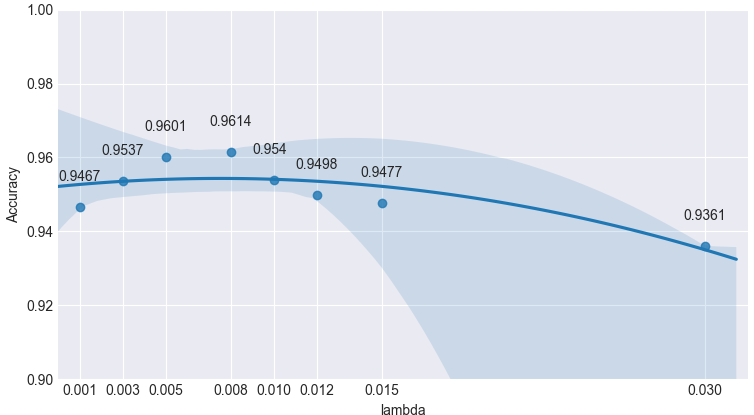
\includegraphics[width=0.9\columnwidth]{perf1.png}
	\caption{Result of $\lambda$ Tuning} \label{fig:perf1}
\end{figure}

From the regression curve, it is observed that the best $\lambda$ value is around $0.008$.

%% 
\subsection{\large Influence of Training Data Size}
Choosing $\lambda = 0.008$ according to the result of previous section, the \textit{Accuracy} result shows a positive relation with the number of training data $numTrainee$, as shown in Table \ref{tab:perf2} and Figure \ref{fig:perf2}. Result of every $numTrainee$ is obtained by taking mean of $5$ tests.
\vspace{8pt}
\begin{table}[H]
	\centering
	\begin{tabular}{c||ccccc}
		\thickhline
		$numTrainee$ & 5 & 10 & 20 & 30 & 40 \\
		\textit{Accuracy} & 0.6484 & 0.8130 & 0.9140 & 0.9421 & 0.9614 \\ \thickhline
	\end{tabular}
	\vspace{6pt}
	\caption{Relation between $numTrainee$ and \textit{Accuracy}} \label{tab:perf2}
\end{table}
\begin{figure}[H]
	\centering
	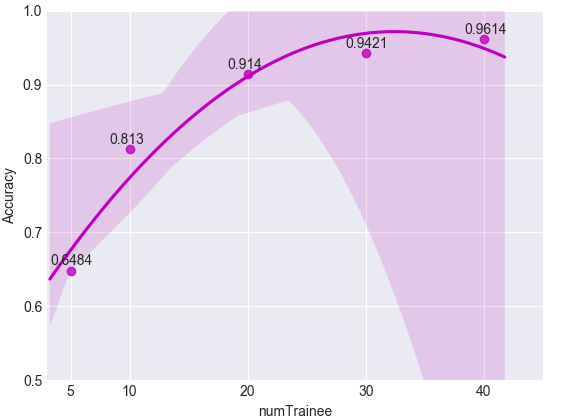
\includegraphics[width=0.8\columnwidth]{perf2.png}
	\caption{Relation between $numTrainee$ and \textit{Accuracy}} \label{fig:perf2}
\end{figure}

%% 
\subsection{\large Run Time Comparison}
Run time of principle component analysis procedure under different number of input data shows great discrepency between official pca() function, which invokes an economic Singular Value Decomposition (SVD), and my self-written fast PCA() accomplishment, as shown in Table \ref{tab:perf3}.
\vspace{8pt}
\begin{table}[H]
	\centering
	\begin{tabular}{c||cc}
		\thickhline
		$numTrainee$ & Official pca() & My Fast PCA() \\ \hline
		5 & 1.09s & 0.12s \\ 
		10 & 2.31s & 0.31s \\ 
		20 & 5.00s & 0.90s \\ 
		30 & 8.39s & 1.79s \\ 
		40 & 13.41s & 3.06s \\ \thickhline
	\end{tabular}
	\vspace{6pt}
	\caption{Run Time Comparison of PCA} \label{tab:perf3}
\end{table}

% Conclusions
\section{\textbf{\large Observations}}
There are several details of this algorithm that can get improved in the future, as listed below:
\begin{itemize}
	\item \textbf{Higher Accuracy by Better Normalization}
	\item \textbf{Image Resizing for Larger Inputs}
	\item \textbf{Adjustments for Illumination and Position}
\end{itemize}

%% 
\subsection{Higher Accuracy by Better Normalization}
Inspired by the report written by Haocong Luo and Yang Zhou, I realize that simply normalize the input images by dividing L2-Norm is not the best approach of normalization. According to their experiments, High Contrast Histogram Equalization is a much better pre-process operation, which brings the \textit{Accuracy} result up to $0.99$.

%% 
\subsection{Image Resizing for Larger Inputs}
For larger image inputs, the computation complexity could increase rapidly. Therefore, a resizing operation is need before reading in all the images. Different compressing methods, including \textit{nearest interpolation}, \textit{bilinear interpolation}, \textit{bicubic interpolation} or other waveform filters can vary in performance, and is worth testing.

%% 
\subsection{Adjustments for Illumination and Position}
This algorithm relies on a standard dataset where face in each image in the centered position. If the input images are biased, a face position detection procedure is needed. Also, even though this dataset contains images of different illumination conditions for each individual, there could be better methods for amending the effect of extreme illuminations.

% Acknowledgment
\section*{\textbf{\large Acknowledgment}}
During this project, I used dataset $CroppedYale$ from Yale. I discussed the idea of PCA and Accuracy testing with Ruoyu Wang, Haoyi Zhu and Xinyu Zhang. I also referred to CSDN blogs \cite{csdn1}, paper from MII \cite{cnki1} and report written by YangZhou \cite{report1} and Haocong Luo \cite{report2}.

% References
\bibliographystyle{IEEEtran}
\bibliography{Reference}

\end{document}
